% ~500 words
% Structure: OER challenge → LiaScript approach (with quiz example) →
%            blind spot → research questions

The creation of high-quality Open Educational Resources remains a persistent
challenge in higher education.
While content management systems and dedicated authoring tools exist,
they often impose significant technical barriers or proprietary lock-in,
discouraging educators from investing in interactive, reusable
materials~\cite{Henderson2018}.

\subsection{The LiaScript Approach}

LiaScript~\cite{Dietrich2019} takes a different approach: it extends standard
Markdown with interactive and multimedia elements using a human-readable syntax.
Listing~\ref{lst:quiz} illustrates this principle: a single-choice quiz
is expressed as a simple list with bracketed markers, directly within the
Markdown source.

\begin{figure}[ht]
  \begin{minipage}[t]{0.46\textwidth}
\begin{verbatim}
Where does DELFI 2026 take place?

- [( )] Munich
- [(X)] Potsdam
- [( )] Hamburg
[[?]] It is the capital of Brandenburg.
***
Potsdam hosts DELFI 2026 together
with HDI at the University of Potsdam.
***
\end{verbatim}
  \end{minipage}%
  \hfill
  \begin{minipage}[t]{0.50\textwidth}
    \vspace{0pt}
    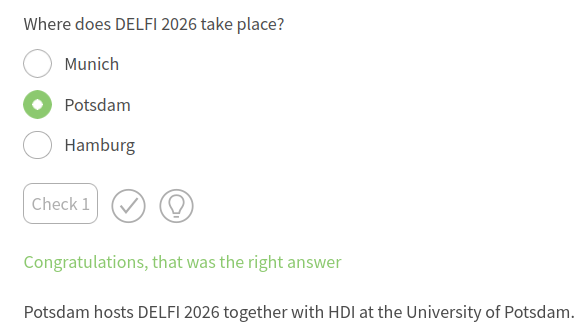
\includegraphics[width=\textwidth]{static_figures/Screenshot.png}
  \end{minipage}
  \caption{A LiaScript single-choice quiz: Markdown source (left) and
           rendered output (right).}
  \label{lst:quiz}
\end{figure}

Beyond quizzes, the language supports text-to-speech narration, animations,
executable code environments, reusable macro libraries, and many more
didactic elements --- all authored as plain text.
Unlike H5P, which requires a server and a Moodle/WordPress installation,
or Jupyter Book,
LiaScript executes without backend infrastructure.
A course file is a standard \texttt{.md} file; the LiaScript interpreter
is loaded client-side via a single URL.
An author pushes the file to any public Git host
and shares a link of the form \texttt{https://liascript.github.io/course/?URL}.
The browser fetches the file and interprets it locally;
no data is sent to any LiaScript server.

This client-side architecture is a deliberate design choice with significant
advantages: courses can be hosted anywhere, require no accounts, respect
learner privacy, and remain accessible even offline.
However, it introduces a fundamental blind spot for the developers.
Because no requests pass through a central server, \emph{there is no telemetry}.
The developers cannot observe which features are used, which courses are
accessed, or whether the pedagogical affordances built into the language
are exploited in practice.

\subsection{Contribution and Research Questions}

The only observable proxy for actual usage is the set of publicly available
LiaScript courses on GitHub.
This paper exploits that proxy systematically.
We analyse a corpus of \num{3317} validated courses from \num{307} committers,
introducing a didactically motivated taxonomy of LiaScript features and mapping
actual adoption rates onto the designed feature space.
The result is the first empirical picture of how LiaScript is used in the wild.

A key methodological choice is the segmentation of the corpus into three
groups: the LiaScript core developers (Internal), a prolific school-focused
power user (MINT-the-GAP), and the broader community.
This separation prevents the highly atypical output of the first two groups
from distorting aggregate adoption statistics.

Concretely, we address three research questions:
\begin{description}
  \item[RQ\,1] Which LiaScript features are adopted by the community and
               which remain underutilised?
  \item[RQ\,2] How do Internal, MINT-the-GAP, and Community groups differ
               in their feature adoption profiles?
  \item[RQ\,3] What development and documentation priorities follow from
               the identified adoption gaps?
\end{description}

The remainder of the paper is structured as follows.
Section~\ref{sec:background} reviews related work on OER tools, feature
adoption, and repository mining.
Section~\ref{sec:methodology} describes the feature taxonomy, the corpus,
and the three-group segmentation.
Section~\ref{sec:adoption} presents the empirical results.
Section~\ref{sec:implications} derives development priorities from the
identified adoption gaps, and
Section~\ref{sec:conclusion} summarises the contributions.
